En este cap\'itulo se describe el desarrollo del proyecto. En primer lugar, se verá el entorno general del proyecto, explicando a grandes rasgos como funciona el proyecto en conjunto. Luego se explica la construcci\'on del interfaz de usuario en Unity, donde interviene de forma directa el sistema de interacci\'on cerebro - computador. A continuaci\'on se describe el desarrollo del sistema controlado, en este caso un Pan - Tilt equipado con una c\'amara. El control del sistema Pan-Tilt implica el desarrollo de una aplicaci\'on ESP-IDF para un ESP32 montado en una targeta de desarrollo. La aplicaci\'on de la c\'amara inteligente no forma parte de este proyecto de fin de grado, por lo que no se describe aqu\'i aunque s'i se enumeran los requisitos que debe cumplir en relaci\'on a las dem\'as partes del proyecto.

\section{Entorno general del proyecto}
\label{section:generalenvironment}

Una vez instalado todo el entorno correctamente (véase , es el momento de explicar cómo se integran todos los componentes para poner en funcionamiento el proyecto.



La figura \ref{figure:diagram-ros2forunity} presenta un diagrama que representa la visión general del sistema.



Es importante mencionar que todos los componentes de ROS 2 deben estar dentro de la misma red. De esta forma, Unity puede conectarse a la red en la que se está ejecutando el agente de micro-ROS. Esta red es generada por el microcontrolador ESP32, que actúa como punto de acceso.



\begin{figure}[!htb]
\centering
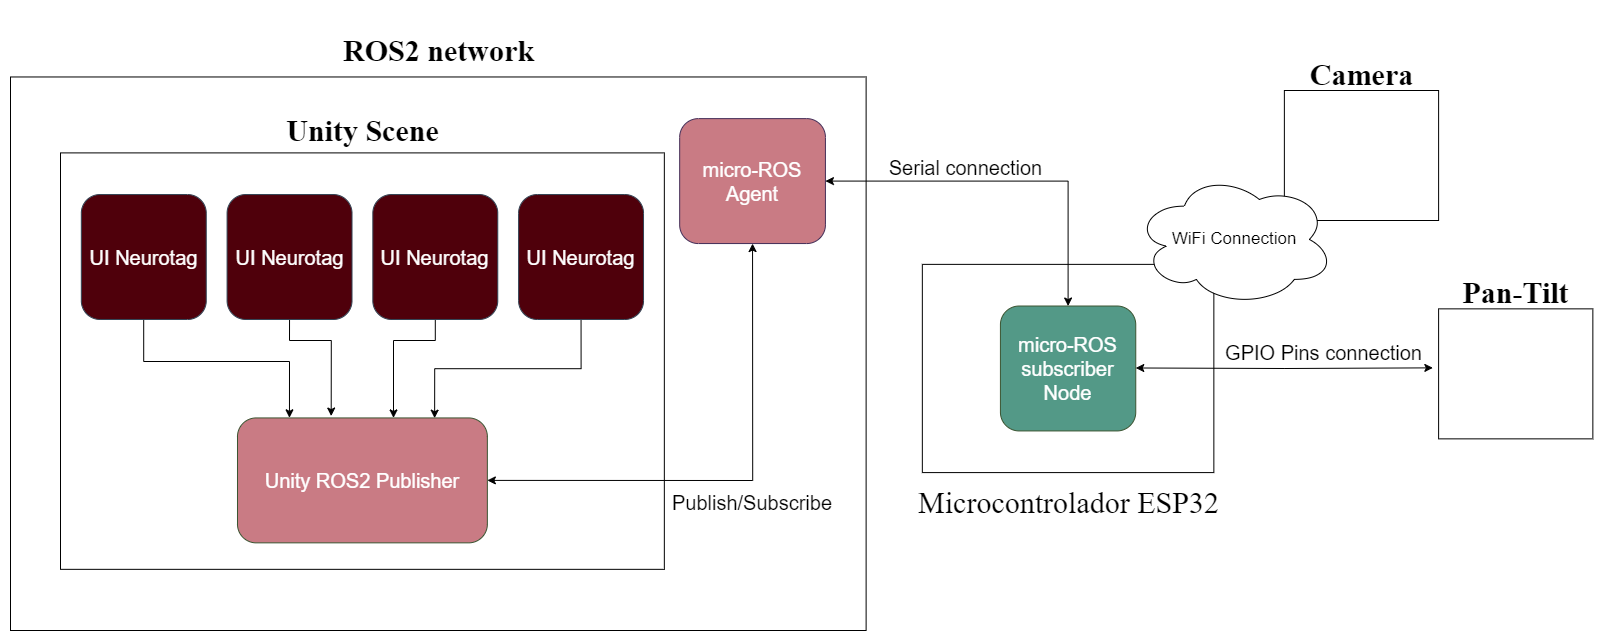
\includegraphics[width=1\linewidth]{figures/Diagram-Ros2ForUnity.png}
\caption{Diagrama del funcionamiento del sistema}
\label{figure:diagram-ros2forunity}
\end{figure}
% Añadir el topic action entre el Publisher y micro-ROS



Con ayuda de la librería Ros2ForUnity, Unity crea un nodo publicador de ROS2 que publica en el tópico ``action''. Un tópico o topic en ROS es un nombre que se utiliza para identificar un canal de comunicación a través del cual los nodos pueden publicar o suscribirse a mensajes.

El nodo suscriptor en el microcontrolador ESP32 se suscribe a este mismo tópico, lo que le permite integrarse en la red de ROS2 a través del agente que se está ejecutando.



Una vez que se ha establecido la comunicación entre Unity y el ESP32, el microcontrolador recibe los mensajes que el nodo publicador transmite a través de ROS2, lo que le permite actuar en consecuencia para controlar el sistema Pan-Tilt y la cámara.



Para garantizar la correcta comunicación, se ha creado un nodo suscriptor en Unity y un nodo publicador en el ESP32 (no representados en el diagrama). Ambos nodos están adscritos al tópico ``freertos\_header\_log'', lo que permite el control de errores. También se ha acabado usando como controlador de la cámara y para que el ESP32 envíe la IP de la cámara a Unity y que este no tenga que saberla de antemano. Gracias a esto Unity no necesita a priori saber su IP sino que será guardada automáticamente cuando la cámara se conecte.
